% ****** Start of file apssamp.tex ******
%
%   This file is part of the APS files in the REVTeX 4.2 distribution.
%   Version 4.2a of REVTeX, December 2014
%
%   Copyright (c) 2014 The American Physical Society.
%
%   See the REVTeX 4 README file for restrictions and more information.
%
% TeX'ing this file requires that you have AMS-LaTeX 2.0 installed
% as well as the rest of the prerequisites for REVTeX 4.2
%
% See the REVTeX 4 README file
% It also requires running BibTeX. The commands are as follows:
%
%  1)  latex apssamp.tex
%  2)  bibtex apssamp
%  3)  latex apssamp.tex
%  4)  latex apssamp.tex
%
\documentclass[%
 reprint,
 superscriptaddress,
%groupedaddress,
%unsortedaddress,
%runinaddress,
%frontmatterverbose, 
%preprint,
%preprintnumbers,
 nofootinbib,
%nobibnotes,
%bibnotes,
 amsmath,amssymb,
 aps,
%pra,
%prb,
%rmp,
%prstab,
%prstper,
%floatfix,
]{revtex4-2}

\usepackage{graphicx}% Include figure files
\usepackage{dcolumn}% Align table columns on decimal point
\usepackage{bm}% bold math
\usepackage{hyperref}% add hypertext capabilities
\usepackage{xcolor}

%\usepackage[showframe,%Uncomment any one of the following lines to test 
%%scale=0.7, marginratio={1:1, 2:3}, ignoreall,% default settings
%%text={7in,10in},centering,
%%margin=1.5in,
%%total={6.5in,8.75in}, top=1.2in, left=0.9in, includefoot,
%%height=10in,a5paper,hmargin={3cm,0.8in},
%]{geometry}

% % % % % % % % % % % % % % % % % % % % % % % % % % % % % %

% journals
\newcommand{\mnras}{MNRAS}
\newcommand{\aap}{A\&A}
\newcommand{\aaps}{A\&AS}
\newcommand{\apjs}{ApJS}
\newcommand{\apjl}{ApJL}
\newcommand{\araa}{ARA\&A}
\newcommand{\jhep}{JHEP}
\newcommand{\aj}{AJ}
\newcommand{\jcap}{JCAP}
\newcommand{\pasp}{PASP}
\newcommand{\pnas}{PNAS}
\newcommand{\epjc}{EPJC}
\newcommand{\nphysa}{Nucl. Phys. A}

% maths
%\newcommand{\dataset}{\vect{d}}
\newcommand{\msun}{M_\odot}
\newcommand{\hubble}{\ensuremath{H_0}}
\newcommand{\hubbleest}{\ensuremath{\hat{H}_0}}
\newcommand{\decel}{\ensuremath{q_0}}
\newcommand{\jerk}{\ensuremath{j_0}}
\newcommand{\dl}{\ensuremath{D}}
\newcommand{\vobs}{\ensuremath{\hat{v}}}
\newcommand{\vobss}{\ensuremath{\hat{\vect{v}}}}
\newcommand{\zobs}{\ensuremath{\hat{z}}}
\newcommand{\zmax}{\ensuremath{z_{\rm max}}}
\newcommand{\prob}{\ensuremath{{\rm P}}}
\newcommand{\normal}{{\rm{N}}}
\newcommand{\sels}{\vect{S}}
\newcommand{\inc}{\iota}
\newcommand{\nexp}{\bar{N}}
\newcommand{\abh}{a_{\rm BH}}
\newcommand{\ans}{a_{\rm NS}}
\newcommand{\mbh}{m_{\rm BH}}
\newcommand{\mns}{m_{\rm NS}}
\newcommand{\mchirp}{{\cal{M}}}
\newcommand{\strain}{h}
\newcommand{\strainobs}{\hat{h}}
\newcommand{\sigmav}{\sigma_{||}}
\newcommand{\gwpoppar}{\beta}
\newcommand{\uniform}{{\rm U}}
\newcommand{\tobs}{t_{\rm obs}}
\newcommand{\fobs}{\Delta_{\rm obs}}
\newcommand{\rate}{\Gamma}
\newcommand{\step}{\Theta}
\newcommand{\snr}{\rho}
\newcommand{\snrmin}{\rho_*}
\newcommand{\mejmin}{m_{\rm ej}^*}
\newcommand{\dgw}{\hat{\bm{x}}}
\newcommand{\kmsmpc}{\ensuremath{{\rm km\,s^{-1}\,Mpc^{-1}}}}
\newcommand{\kms}{\ensuremath{{\rm km\,s^{-1}}}}
\newcommand{\mpc}{\ensuremath{{\rm Mpc}}}
\newcommand{\gpc}{\ensuremath{{\rm Gpc}}}
\newcommand{\yr}{\ensuremath{{\rm yr}}}
\newcommand{\yrgpc}{\ensuremath{{\rm yr^{-1}\,Gpc^{-3}}}}
\newcommand{\planck}{{\it Planck}}
\newcommand{\plancks}{{\it Planck{\rm 's}}}
\newcommand{\lcdm}{$\Lambda$CDM}

% waveforms
\newcommand{\seobnr}{\texttt{SEOBNR}}
\newcommand{\seobnrfull}{\texttt{SEOBNRv4\_ROM\_NRTidalv2\_NSBH}}
\newcommand{\imrp}{\texttt{IMRPhenom}}
\newcommand{\imrpfull}{\texttt{IMRPhenomPv2\_NRTidal}}

% % % % % % % % % % % % % % % % % % % % % % % % % % % % % %

\begin{document}

\title{Prospects for Measuring the Hubble Constant with Neutron-Star-Black-Hole Mergers - Supplemental Material}

\author{Stephen M. Feeney}
\affiliation{Department of Physics \& Astronomy, University College London, Gower Street, London WC1E 6BT, UK}
\author{Hiranya V. Peiris}
\affiliation{Department of Physics \& Astronomy, University College London, Gower Street, London WC1E 6BT, UK}
\affiliation{Oskar Klein Centre for Cosmoparticle Physics, Department of Physics,
Stockholm University, AlbaNova, Stockholm SE-106 91, Sweden}
\author{Samaya M. Nissanke}
\affiliation{GRAPPA, Anton Pannekoek Institute for Astronomy and Institute of High-Energy Physics, University of Amsterdam, Science Park 904, 1098 XH Amsterdam, The Netherlands}
\affiliation{Nikhef, Science Park 105, 1098 XG Amsterdam, The Netherlands}
\author{Daniel J. Mortlock}
\affiliation{Astrophysics Group, Imperial College London, Blackett Laboratory, Prince Consort Road, London SW7 2AZ, UK}
\affiliation{Department of Mathematics, Imperial College London, London SW7 2AZ, UK}
\affiliation{Department of Astronomy, Stockholm University, AlbaNova, SE-10691 Stockholm, Sweden}

\date{\today}% It is always \today, today,
             %  but any date may be explicitly specified

\maketitle

% % % % % % % % % % % % % % % % % % % % % % % % % % % % % %

\textbf{\emph{Waveform Approximants.}} The waveform approximants used in this work are based on the two main methods that model fully the inspiral-merger-ringdown phases of binary black holes. Both models extend the analytically--derived inspiral to incorporate the merger and ringdown by calibrating the full waveforms with a suite of numerical relativity simulations. With these baseline binary black hole models in hand, the two approaches treat the finite-size effects of neutron stars by adding tidal deformation, using BNS numerical relativity simulations, and spin-quadrupole corrections to the GW phase evolution in the waveforms. Specifically, \imrp\ uses a phenomenological approach when extending the post-Newtonian approximation of the inspiral using numerical relativity simulations, which encapsulates the dominant effects of generic precessing binary black holes ~\cite[e.g.,][]{Ajith_etal:2007,*Ajith_etal:2008,*Hannametal:2014}. Importantly, \imrp\ models the merger frequency of the system with a taper for BNS systems only. In contrast, \seobnr\ is based on the Effective-One-Body (EOB) formalism to model the two body problem in General Relativity~\cite[e.g.,][]{Buonanno_Damour:1999, *Buonanno_Damour:2000, *Bohe_etal:2017, *Barausse_Buonanno:2010}. \seobnr\ specifically applies to NSBH systems where the BH spin is aligned or anti-aligned to the orbital angular momentum plane. In addition to the finite-size-induced GW phase correction, \seobnr\ automatically describes the merger frequency for mass ratios of 1--5 using numerical relativity simulations of NSBHs. An updated, NSBH-specific waveform, \texttt{IMRPhenomNSBH}, was released in Ref.~\cite{Thompson_etal:2020}; however, we do not use it here as it is only valid for BH spin magnitudes up to 0.5.

\begin{figure*}[ht!]
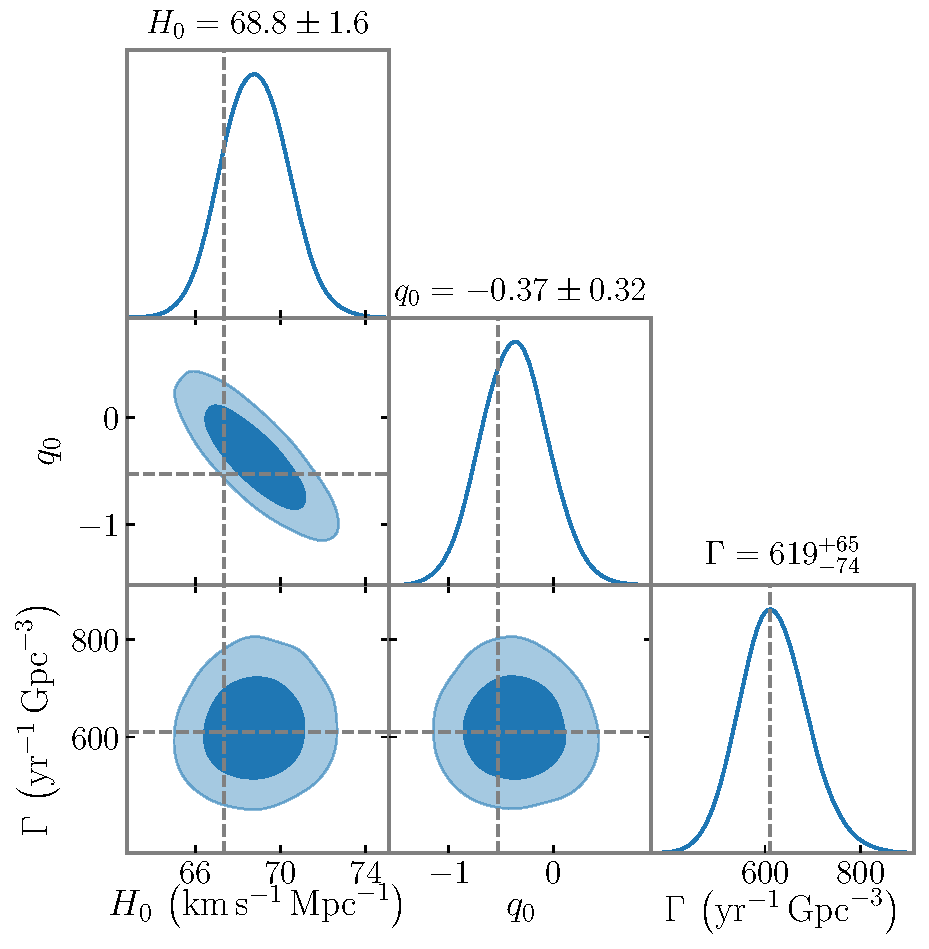
\includegraphics[width=8cm]{fig_3a.pdf}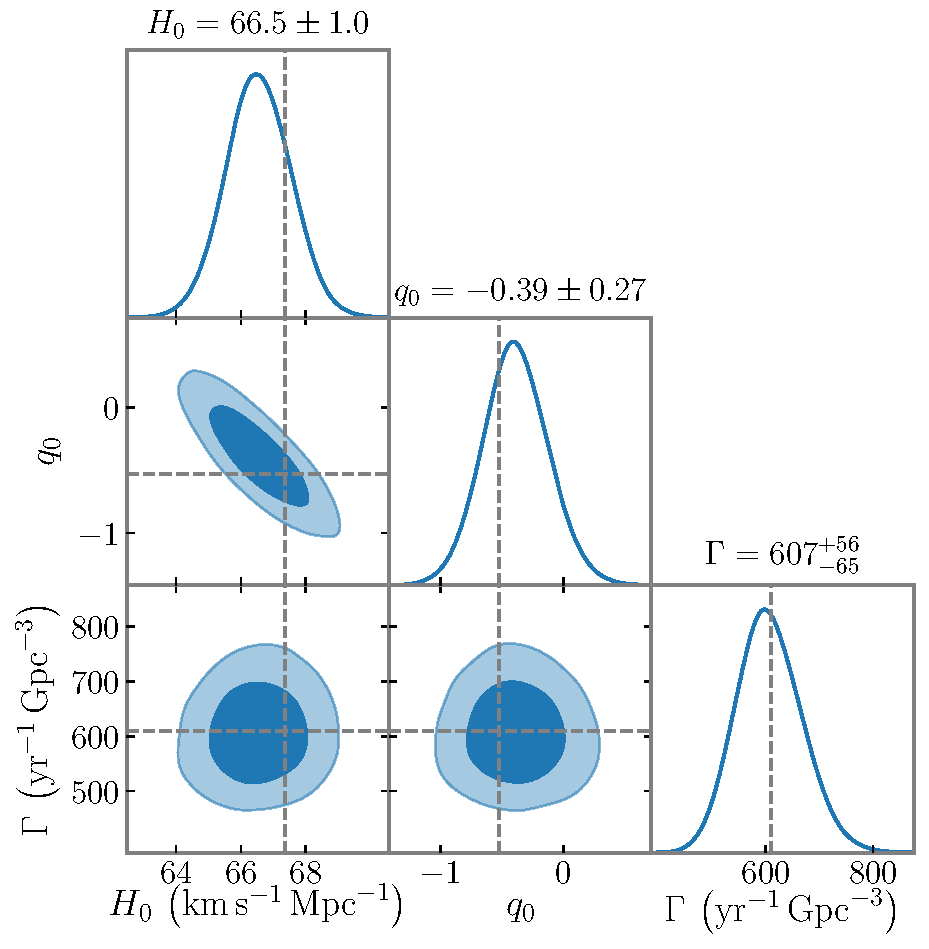
\includegraphics[width=8cm]{fig_3b.pdf}
\caption{Cosmological and population parameter posteriors inferred for the mock \seobnr\ (left) and \imrp\ (right) catalogs.\label{fig:cosmo}}
\end{figure*}

\textbf{\emph{Cosmography.}} We assume a cosmographic distance-redshift relation based on Taylor expanding the relevant quantities to third order in expansion parameters, i.e., the Hubble constant, \hubble, the deceleration parameter, \decel, and the jerk, $j_0$ (which we assume to be one throughout). The luminosity distance is then related to the expansion parameters by~\cite{Visser:2004}
\begin{equation}
d \simeq \frac{cz}{\hubble} \left[1 + \frac{1}{2} \left(1 - \decel \right) z + \frac{1}{6} \left(-1 + \decel - \jerk + 3 \decel^2 \right) z^2 \right],
\label{eq:distance}
\end{equation}
and the comoving volume element by
\begin{align}
\frac{{\rm d}V}{{\rm d}z} \simeq & 4\pi \frac{c^3 z^2}{\hubble^3} \times \label{eq:volel} \\
& \left[1 - 2 \left(1 + \decel \right) z + \frac{5}{12} \left(7 + 14 \decel - 2 \jerk + 9 \decel^2 \right) z^2 \right]. \nonumber
\end{align}
The redshifted volume is defined to be 
\begin{equation}
V = 4\pi \int_0^{\zmax} \frac{{\rm d}V}{{\rm d}z} \frac{{\rm d}z}{1+z}.
\label{eq:volume}
\end{equation}

\textbf{\emph{Posterior.}} Our two-stage Bayesian inference pipeline requires us to first evaluate, for each merger in turn, the GW likelihood marginalized over all parameters $\boldsymbol{\theta}_i$ other than the luminosity distance $d$ to the merger:
\begin{equation}
\prob(\dgw_i | d[ z_i, \hubble, \decel ]) = \int {\rm d}\boldsymbol{\theta}_i \prob(\boldsymbol{\theta}_i) \prob(\dgw_i | d[ z_i, \hubble, \decel ], \boldsymbol{\theta}_i).
\label{eq:marge_like}
\end{equation}
$\dgw_i$ here are the the $i^{\rm th}$ merger's GW strain observations, and $\boldsymbol{\theta}_i$ comprises the merger's component masses, spin magnitudes and orientations (if using precessing spins), inclination, polarization angle, NS tidal deformability, and time and phase at coalescence. With these in hand, the joint posterior of the cosmological and NSBH parameters is given by
\begin{align}
\prob & \left( \hubble, \decel, \Gamma, \{z, v\} | N, \left\{ \dgw, \hat{z}, \hat{v} \right\}, \snrmin, \mejmin \right) \propto \label{eq:posterior} \\
& \prob \left( \hubble, \decel, \Gamma \right) \exp \left( -\bar{N} \left[ \hubble, \decel, \Gamma, \snrmin, \mejmin \right] \right) \times \nonumber \\
& \prod_{i = 1}^{N} \frac{\Gamma}{1 + z_i} \frac{{\rm d}V}{{\rm d}z} \left[ \hubble, \decel \right] \prob (\dgw_i | d \left[ z_i, \hubble, \decel \right]) \prob(v_i) \prob(\hat{v}_i | v_i) \prob(\hat{z}_i | z_i), \nonumber
\end{align}
where $N$ and $\nexp$ are the actual and expected number of mergers detected, respectively, curly brackets denote sets of quantities and bold denotes per-merger vectors. The specific posteriors we obtain after processing our simulated catalogs are shown in Fig.~\ref{fig:cosmo}.

% % % % % % % % % % % % % % % % % % % % % % % % % % % % % %

\bibliography{references}% Produces the bibliography via BibTeX.

\end{document}
%
% ****** End of file apssamp.tex ******